\documentclass[tikz,border=12pt]{standalone}
\usepackage[T1]{fontenc}
\usepackage{mathpazo}
\usepackage{amsmath,amssymb}
\usetikzlibrary{arrows.meta, calc}

\definecolor{stblue}{HTML}{7B97AD}
\definecolor{rwgold}{HTML}{B8995E}
\definecolor{sage}{HTML}{7A9A7E}
\definecolor{dkbrown}{HTML}{3D3530}
\definecolor{wmgray}{HTML}{7B7067}
\definecolor{cream}{HTML}{F9F6F0}
\definecolor{border}{HTML}{D4C9B8}
\definecolor{terracotta}{HTML}{C47A6A}
\definecolor{lavender}{HTML}{907EA0}

\begin{document}
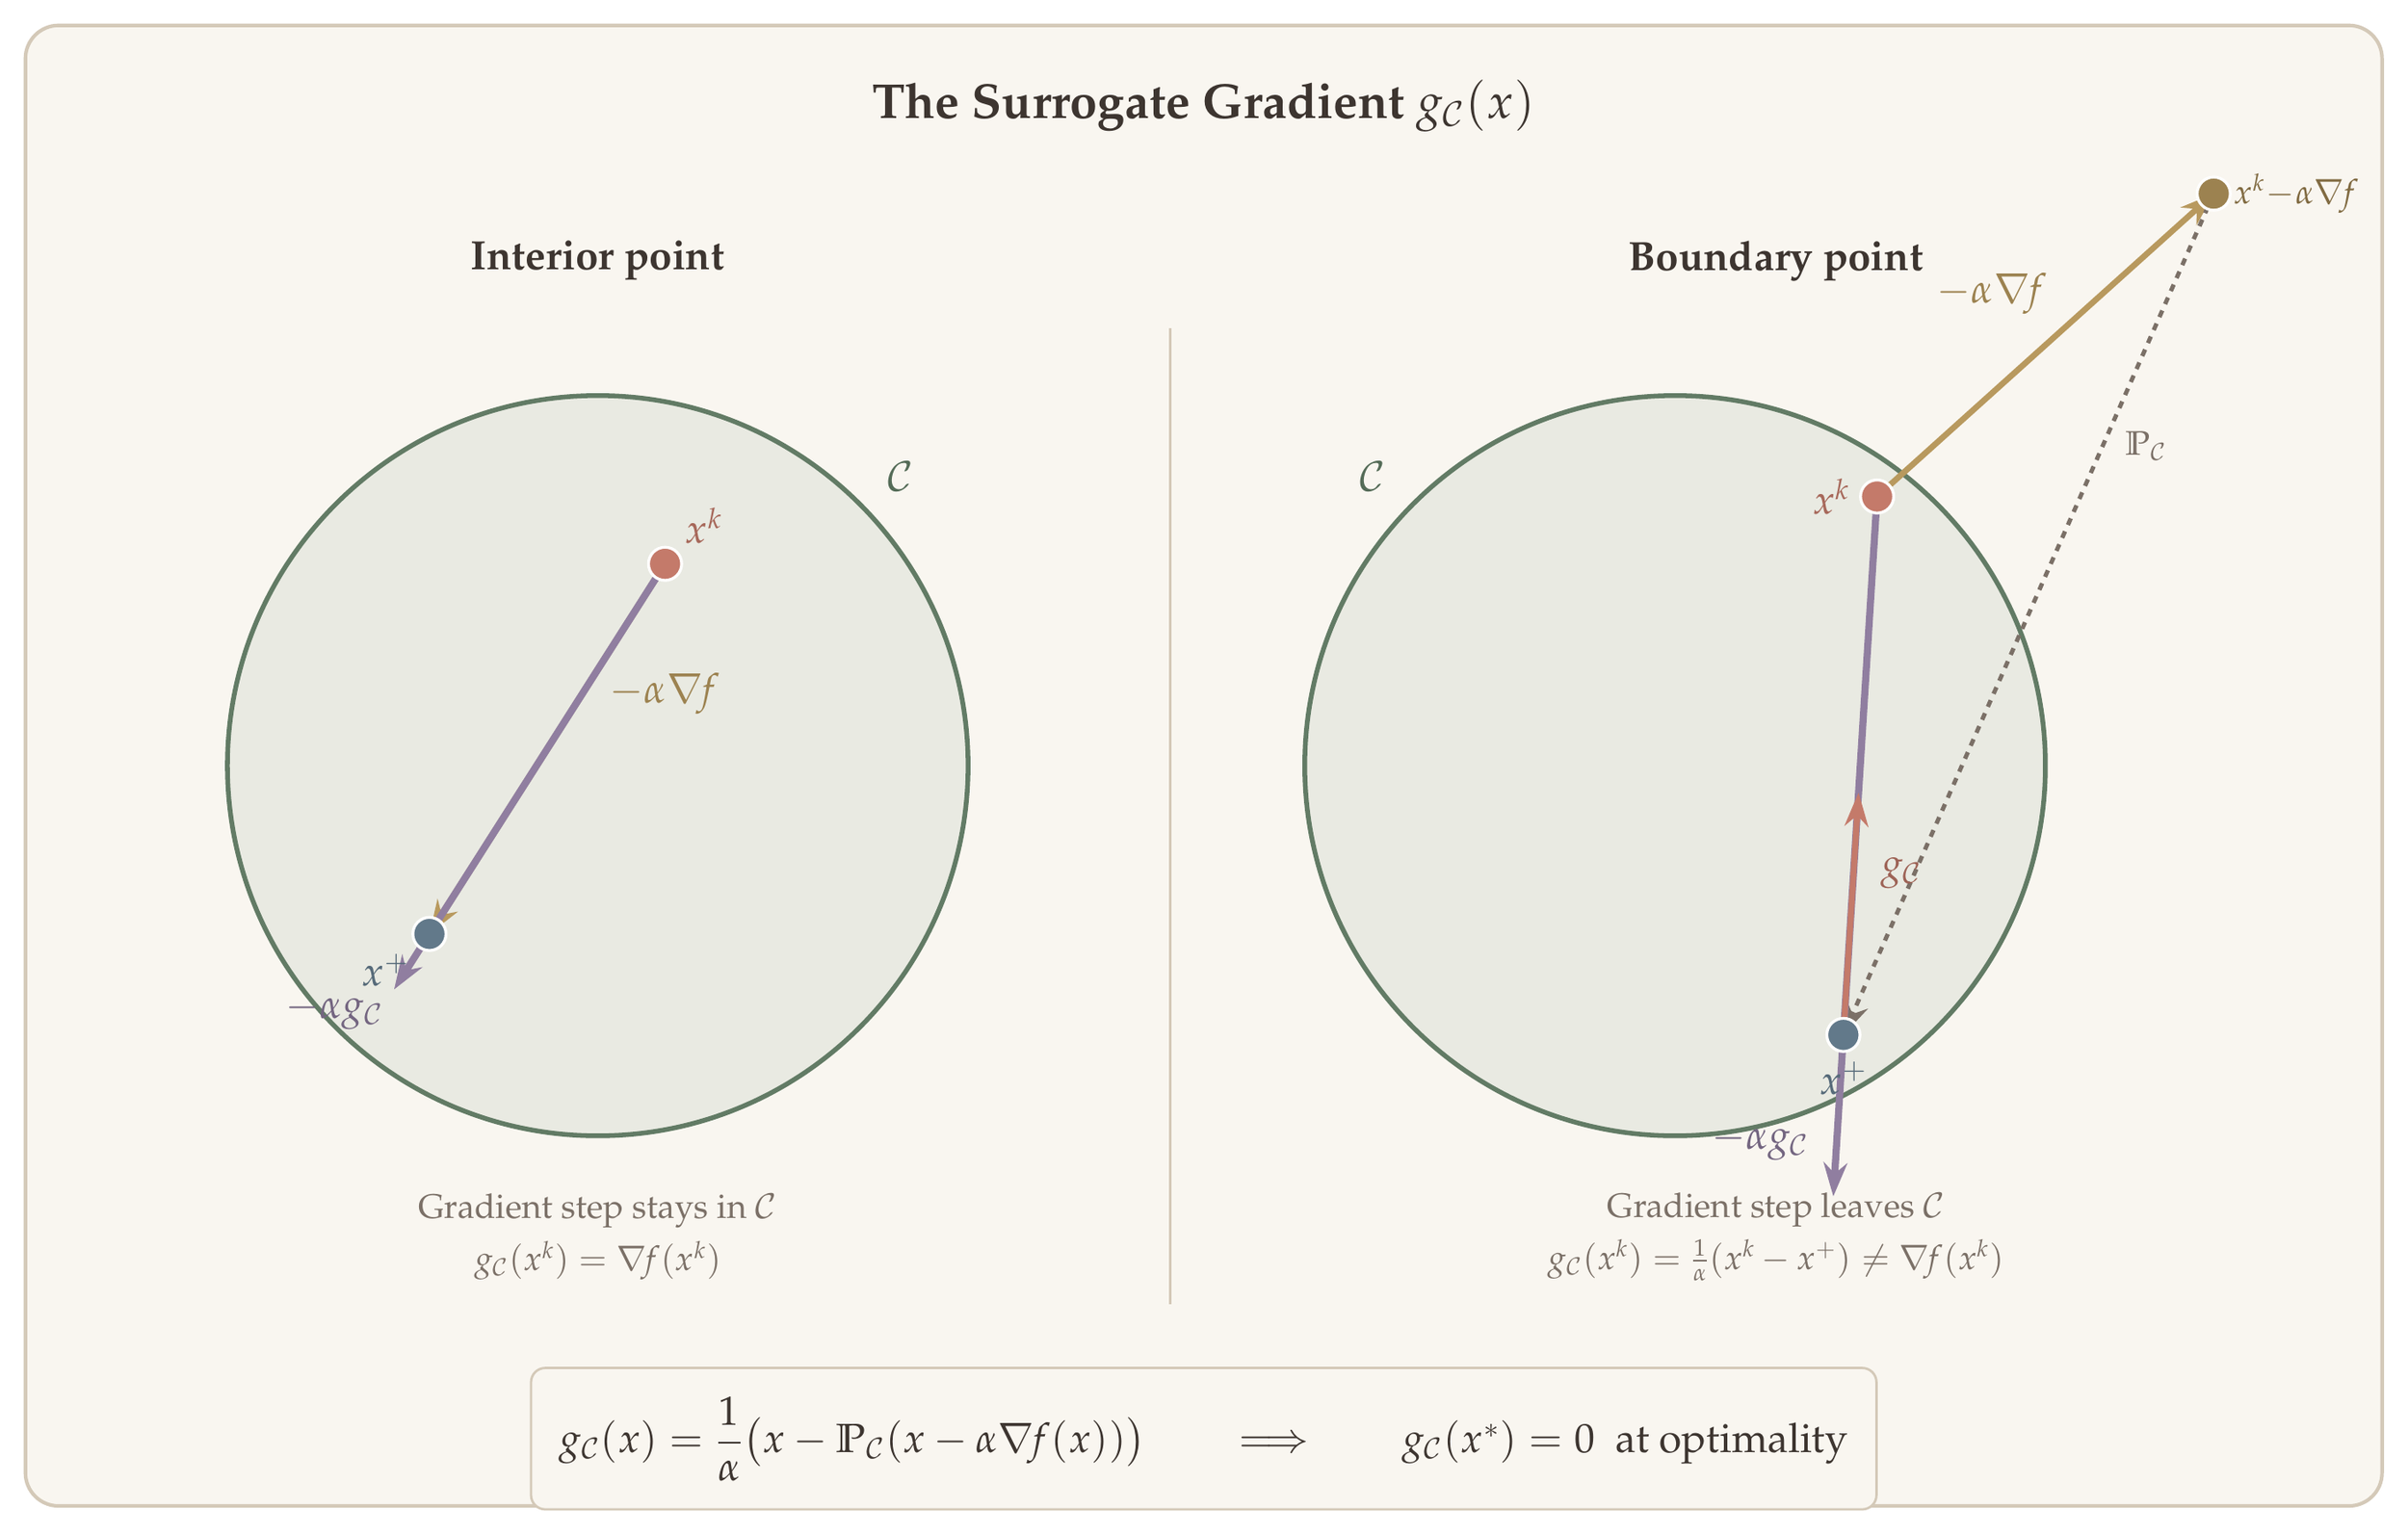
\begin{tikzpicture}[>={Stealth[length=5mm, width=3.5mm]}]

% Background
\fill[cream, rounded corners=14pt] (-2.5,-5.5) rectangle (32.5,16.5);
\draw[border, line width=1.5pt, rounded corners=14pt] (-2.5,-5.5) rectangle (32.5,16.5);

% Title
\node[text=dkbrown, font=\huge\bfseries] at (15.0,15.3)
  {The Surrogate Gradient $g_{\mathcal{C}}(x)$};

% ================================================================
% LEFT PANEL: Interior point (gradient step stays in C)
% ================================================================
\node[text=dkbrown, font=\LARGE\bfseries] at (6.0,13.0) {Interior point};

% Convex set (large circle)
\fill[sage, opacity=0.12] (6.0,5.5) circle (5.5cm);
\draw[sage!80!black, line width=2pt] (6.0,5.5) circle (5.5cm);
\node[text=sage!70!black, font=\LARGE\bfseries] at (10.5,9.8) {$\mathcal{C}$};

% Point x^k (interior, upper area)
\coordinate (xk-L) at (7.0,8.5);
% Gradient step lands inside C (well-separated, lower-left)
\coordinate (gs-L) at (3.5,3.0);

% Gradient step arrow (rwgold)
\draw[rwgold, line width=2.8pt, ->]
  (xk-L) -- (gs-L);
\node[text=rwgold!85!black, font=\LARGE, right=8pt]
  at ($(xk-L)!0.35!(gs-L)$) {$-\alpha\nabla\!f$};

% Surrogate gradient direction (same as gradient here)
\draw[lavender, line width=3pt, ->]
  (xk-L) -- ($(xk-L)!1.15!(gs-L)$);
\node[text=lavender!80!black, font=\LARGE, below left=6pt]
  at ($(xk-L)!1.10!(gs-L)$) {$-\alpha g_{\mathcal{C}}$};

% Points
\fill[terracotta] (xk-L) circle (7pt);
\draw[white, line width=1.2pt] (xk-L) circle (7pt);
\node[text=terracotta!85!black, font=\LARGE\bfseries, above right=5pt]
  at (xk-L) {$x^k$};

\fill[stblue!80!black] (gs-L) circle (7pt);
\draw[white, line width=1.2pt] (gs-L) circle (7pt);
\node[text=stblue!70!black, font=\LARGE, below left=5pt]
  at (gs-L) {$x^+$};

% Caption
\node[text=wmgray, font=\Large, align=center] at (6.0,-1.5)
  {Gradient step stays in $\mathcal{C}$\\[4pt]
   $g_{\mathcal{C}}(x^k) = \nabla\!f(x^k)$};

% ================================================================
% RIGHT PANEL: Boundary point (gradient step leaves C)
% ================================================================
\node[text=dkbrown, font=\LARGE\bfseries] at (23.5,13.0) {Boundary point};

% Convex set (large circle)
\fill[sage, opacity=0.12] (22.0,5.5) circle (5.5cm);
\draw[sage!80!black, line width=2pt] (22.0,5.5) circle (5.5cm);
\node[text=sage!70!black, font=\LARGE\bfseries] at (17.5,9.8) {$\mathcal{C}$};

% Point x^k (on the boundary, upper-right of circle)
\coordinate (xk-R) at (25.0,9.5);
% Gradient step goes far outside (upper-right, well separated)
\coordinate (gs-R) at (30.0,14.0);
% Projected point x^+ (back on boundary, lower area)
\coordinate (xp-R) at (24.5,1.5);

% Step 1: Gradient step arrow (goes outside C)
\draw[rwgold, line width=2.5pt, ->]
  (xk-R) -- (gs-R);
\node[text=rwgold!85!black, font=\LARGE, above left=3pt]
  at ($(xk-R)!0.55!(gs-R)$) {$-\alpha\nabla\!f$};

% Step 2: Projection arrow (dashed, from gradient step to x^+)
\draw[wmgray, line width=1.8pt, dashed, ->]
  (gs-R) -- (xp-R);
\node[text=wmgray, font=\Large, right=6pt]
  at ($(gs-R)!0.3!(xp-R)$) {$\mathbb{P}_{\mathcal{C}}$};

% The surrogate gradient direction: from x^k toward x^+ and beyond
\draw[lavender, line width=3pt, ->]
  (xk-R) -- ($(xk-R)!1.30!(xp-R)$);
\node[text=lavender!80!black, font=\LARGE, left=8pt]
  at ($(xk-R)!1.20!(xp-R)$) {$-\alpha g_{\mathcal{C}}$};

% The g_C vector shown from x^+ back toward x^k
\draw[terracotta, line width=2.5pt, ->]
  (xp-R) -- ($(xp-R)!0.45!(xk-R)$);
\node[text=terracotta!80!black, font=\LARGE, right=8pt]
  at ($(xp-R)!0.30!(xk-R)$) {$g_{\mathcal{C}}$};

% Points (drawn last, on top)
\fill[terracotta] (xk-R) circle (7pt);
\draw[white, line width=1.2pt] (xk-R) circle (7pt);
\node[text=terracotta!85!black, font=\LARGE\bfseries, left=8pt]
  at (xk-R) {$x^k$};

\fill[rwgold!85!black] (gs-R) circle (7pt);
\draw[white, line width=1.2pt] (gs-R) circle (7pt);
\node[text=rwgold!70!black, font=\Large, right=5pt]
  at (gs-R) {$x^k\!-\!\alpha\nabla\!f$};

\fill[stblue!80!black] (xp-R) circle (7pt);
\draw[white, line width=1.2pt] (xp-R) circle (7pt);
\node[text=stblue!70!black, font=\LARGE, below=8pt]
  at (xp-R) {$x^+$};

% Caption
\node[text=wmgray, font=\Large, align=center] at (23.5,-1.5)
  {Gradient step leaves $\mathcal{C}$\\[4pt]
   $g_{\mathcal{C}}(x^k) = \tfrac{1}{\alpha}(x^k - x^+) \neq \nabla\!f(x^k)$};

% ================================================================
% Divider line
% ================================================================
\draw[border, line width=1pt] (14.5,-2.5) -- (14.5,12.0);

% ================================================================
% Bottom formula box
% ================================================================
\node[text=dkbrown, font=\LARGE,
      fill=cream, inner sep=12pt,
      draw=border, line width=1pt, rounded corners=6pt]
  at (15.0,-4.5)
  {$g_{\mathcal{C}}(x) = \dfrac{1}{\alpha}\bigl(x - \mathbb{P}_{\mathcal{C}}(x - \alpha\nabla\!f(x))\bigr)
    \qquad\Longrightarrow\qquad g_{\mathcal{C}}(x^*) = 0\ $ at optimality};

\end{tikzpicture}
\end{document}
